\chapter{Sicurezza dei Programmi}
La sicurezza dei programmi è al cuore della sicurezza informatica, in quanto i programmi costituiscono gran parte di un sistema operativo. Sorgono due domande:
\begin{itemize}
\item Come è possibile prevenire la presenza di difetti in un programma?
\item Come è possibile proteggere le risorse informatiche da programmi che contengono difetti?
\end{itemize}

Un programma, che è un insieme di istruzioni per il calcolatore, è detto \textbf{sicuro} se abbiamo un certo grado di fiducia nel fatto che il programma garantisca \underline{riservatezza, integrità e la disponibilità} che ci si apsetta.
Valutare la sicurezza di un software è un procedimento analogo a valutarne la qualità in generale.
\paragraph{Terminologia}
\begin{itemize}
\item \textbf{Difetto (Fault)}: passaggio, comando o definizione dei dati non corretto in un programma
\item \textbf{Malfunzionamento}: deviazione dal comportamento richiesto del sistema
\end{itemize}

Quindi un difetto è un errore dal punto di vista interno, quello del programmatore; mentre un malfunzionamento è un errore dal punto di vista esterno, dell'utente. Perciò un difetto è una causa, il malfunzionamento è un effetto.
\textbf{N.B.} non sempre un difetto si traduce in uno o più malfunzionamenti (il codice difettoso potrebbe non venire mai eseguito).

La qualità di un software dipende dal punto di vista di chi sta analizzando il programma, per questo motivo è possibile avere divergenze nelle accezioni! Un programma può essere sicuro perché:

\begin{itemize}
\item é necessario troppo tempo per la violazione dei protocolli di protezione
\item é stato eseguito per un certo periodo di tempo senza malfunzionamenti 
\item nessun errore è stato riscontrato
\end{itemize}

La sicurezza é per sua natura una questione complessa, che spesso entra in conflitto con usabilità e prestazioni, inoltre non esistono tecniche per eliminare o gestire tutte le falle di sicurezza.
La complessità nel trattare la sicurezza dei programmi è data da:

\begin{itemize}
\item \textbf{Complessità del Sistema}: è quasi impossibile definire tutti i requisiti di sicurezza, in quanto in un sistema grande e articolato le interazioni tra i vari moduli accadono in un numero di modi che non é gestibile. Quindi l'esame e la verifica vengono fatti per i casi più probabili, non esaustivamente. Quindi, la dimensione e la complessità dei sistemi impediscono una prevenzione completa delle falle.
\item \textbf{Evoluzione tecniche di programmazione}: la programmazione e le tecniche di ingegneria del software cambiano e si evolvono molto più rapidamente delle tecniche di sicurezza informatica.
\end{itemize}

\section{Errori di Programma Non Malevoli}
Programmatori e analisti commettono errori, spesso né intenzionali né malevoli. Molti di essi provocano malfunzionamenti, ma non portano a vulnerabilità serie. Alcune classi di errori hanno costituito un grosso problema per la sicurezza e continueranno a costituirlo. 
Di seguito sono riportate alcune di queste classi (saranno trattate solo quelle che non sono state incontrate nei capitoli precedenti):

\begin{itemize}
\item \textbf{Buffer Overflow}
\item \textbf{Mediazione Incompleta}
\item \textbf{Errori dovuti allo scarto fra tempo di controllo e tempo di utilizzo}
\end{itemize}

\subsection{Mediazione Incompleta}
Prendiamo ad esempio un sito Web, il cui indirizzo è:
 http://www.somesite.com/subpage/
  userinput.asp?param1=(808)555-1212\&parm2=2009Jan17.
  \newline
Cosa accadrebbe se fosse specificata un altra data? 
Potrei inserire dei comandi a lato client per impedire il buffer overflow. Ad esempio la data potrebbe essere specificata solo selezionando controlli predefiniti, ciò non impedisce di realizzare una richiesta HTTP manuale e in questo caso si dice che i valori dei dati non sono stati completamente mediati; i dati critici si trovano in una condizione esposta, non controllata.
Per meglio comprendere le implicazioni per la sicurezza consideriamo il seguente esempio:
\begin{itemize}
	\item Supponiamo che la richiesta HTTP per la conferma di pagamento sia la seguente:
	\newline
	http://www.things.com/order.asp?part=555\&price=10\&quantity=5\&total=50
	\item Normalmente un utente utilizza il sito di e-commerce dell'azienda e non genera una richiesta manuale, cioò però non impedisce di confezionare una richiesta malevola come:
	\newline
	http://www.things.com/order.asp?part=555\&price=10\&quantity=5\&total=50
	\item Come si risolve? \`{E} sufficiente avere il codice del prodotto e la quantità, e non il prezzo unitario nè il totale!
\end{itemize}

\subsection{Scarto fra tempo di controllo e tempo di utilizzo}
Per migliorare l'efficenza i processori e sistemi operativi moderni possono cambiare l'ordine di esecuzioni di istruzioni e procedure. Ad esempio l'esecuzione di istruzioni consecutive di una procedura possono essere inframezzate da istruzioni di altre procedure (multi-tasking).
\newline
La falla \textbf{TOCTTOU}(Time Of Check To Time Of Use) è dovuta allo scarto di tempo tra la verifica dell'autorizzazione a compiere un azione e l'esecuzione dell'azione stessa. Se i dati di autorizzazione non vengono utilizzati direttamente e, nell'attesa di essere utilizzati, sono disponibili per la modifica, allora si verifica la falla.
\subparagraph{Ad esempio} se una persona compra una statua che costa 100 \officialeuro, l'acquirente estrae 5 banconote da 20 \officialeuro, le conta davanti al venditore e le lascia sul tavolo. Quando il venditore si gira e prende la statua l'acquirente riprende una banconota, i due finiscono la transazione e l'acquirente esce dal negozio.
Lo stesso, sostanzialmente, può accadere con la richiesta e il rilascio di permessi di accesso ai file. Nel mentre che un permesso viene accordato può essere cambiato dall'entità che lo ha generato, permettendo operazioni negate.
\newline
Per evitare la falla sarebbe necessario utilizzare i dati di permesso immediatamente o evitare di esporli durante l'attesa dell'utilizzo, se ciò non fosse possibile si potrebbe aggiungere un checksum ai dati di permesso che l'entità emittente possa verificare in modo da poter rilevare modifiche.

Ognuna delle tre falle precedenti è abbastanza grave singolarmente, tuttavia l'aggressore intelligente utilizza le falle come mattoni per la costruzione di un attacco complesso.
Per questo motivo occorre conoscere e proteggersi anche dalle falle più semplici, anche le più innocue.

\section{Virus e altro codice malevolo}
La maggior parte del lavoro svolta da un programma è invisibile agli utenti; per questa ragione, poiché l'utente non vede direttamente i dati utilizzati dal computer, gli eventuali aggressori informatici possono utilizzare programmi come veicoli per la modifica di dati o di altri programmi.
\subsection{Installazione e descrizione del codice malevolo}
Quindi, quando si installa un pacchetto software si esegue un comando \textbf{Install} o \textbf{Setup}; da qui in poi il programma di installazione prende il controllo e crea, modifica, elimina e rinomina i file che gli sono necessari.
\newline
A parte la documentazione di installazione fornita, l'utente non ha idea di quali regalini abbia ricevuto in seguito alla installazione. Si spera che siano tutti buoni, ma tra essi è possibile nascondere del codice malevolo che viene installato senza che l'utente ne abbia percezione, per questo è importante consocere la fonte del software che installiamo!

\subsubsection{Cosa può fare il codice malevolo}
Il codice malevolo è di fatto un programma e può quindi fare qualsiasi cosa è in grado di fare un software (scrivere messaggi a schermo, terminare esecuzione di un altro programma, modifica/cancellare dati, etc. etc.).
Può anche insidiarsi e rimanere inattivo fino a che non si verifica una condizione di innesco (un orario, data, eventi interni, conteggio, etc. etc.).
Il codice malevolo viene eseguito sotto l'autorità dell'utente corrente e venire a contatto con tutto ciò è a contatto l'utente allo stesso modo (sebbene non ne sia a conoscenza).
\subsubsection{Da quando esiste il codice malevolo?}
I primi riferimenti ai comportamenti dei virus risalgono al 1970, lo studio di Ware e quello di Anderson per l'aeronautica militare statunitense descrivono in maniera accurata minacce, vulnerabilità e falle di protezione dei programmi.
La novità oggigiorno è il numero di istanze distinte e di copie di virus che sono comparse e scomparse, nonchè la velocità con cui nasce il codice per il loro sfruttamento.

\subsection{Protezione da codice malevolo}
Il rilascio di una patch per tappare una vulnerabilità avviene secondo le seguente fasi
\begin{itemize}
\item Una nuova vulnerabilità viene scoperta
\item Il produttore ne viene a conoscenza
\item Viene sviluppata la prova di concetto per dimostrare la vulnerabilità in una situazione controllata
\item Il produttore sviluppa e distribuisce un rimedio
\item Gli utenti implementano la difesa
\end{itemize}
Qualcuno può sferrare un attacco effettivo estendendo la prova di concetto o la definizione della vulnerabilità, fintanto che gli utenti implementano la difesa prima dell'attacco effettivo, non si registra alcun danno.
Viene definito \textbf{Giorno Zero} la data in cui il produttore viene a conoscenza della vulnerabilità.
Un attacco che avvenga prima che il produttore conosca la vulnerabilità è detto \textbf{zero day attack} ma, in senso più generale, uno zero day attack avviene prima della disponibilità della patch relativa.

\subsection{Tipi di codice malevolo}
Segue un elenco di definizioni e descrizioni dei tipi di codice malevolo
\begin{itemize}

	\item \textbf{Virus}: si unisce ad un programma e propaga copia di se stesso in altri programmi, è di tipo transitorio se eseguito solamente in associazione al programma ospite, residente se rimane sempre attivo e può essere attivato come programma autonomo dopo il termine del programma ospite.
	\item \textbf{Cavallo di Troia}: codice che oltre al suo effetto primario presenta un secondo effetto malevolo non evidente, ad esempio uno script di login che conserva una copia di nome utente e password per utilizzo successivo
	\item \textbf{Bomba logica}: codice malevolo che scatta al verificarsi di una particolare situazione
	\item \textbf{Trapdoor o Backdoor}: caratteristica di un programma per accesso diverso dalla chiamata diretta; ad esempio un programma bancario che, digitando il numero 990099, mostra la registrazione delle operazioni effettuate
	\item \textbf{Worm}: come il Virus, ma si diffonde solo attraverso la rete, mentre il virus può utilizzare qualsiasi supporto. Il worm si diffonde come programma autonomo.
	\item \textbf{Rabbit}: virus o worm che si replica automaticamente senza limiti per poter esaurire le risorse
\end{itemize}

\subsection{Diffusione dei Virus}
Un virus eseguibile semplicemente residente su un disco non produce effetti, affinché il virus inizi il suo lavoro malevolo e si diffonda deve essere attivato attraverso la sua esecuzione. Il virus quindi viene associato ad un programma ospite in modo tale da essere eseguito quanto l'ospite è lanciato.
\subparagraph{Ad esempio} dopo l'avvio di un SETUP.exe, il virus può procedere autonomamente con l'infezione; quindi per cominciare il processo di infezione è necessario un intervento umano.
\newline
Un mezzo comune per la diffusione di virus è la posta elettronica, in questo attacco l'aggressore deve convincere il destinatario del messaggio ad aprire l'allegato, una volta aperto può infettare il pc.
Alcuni gestori di posta elettronica, nel tentativo di aiutare l'utente aprivano direttamente gli allegati alla sola lettura del messaggio, andando a creare una falla di sicurezza.

\subsection{Posizione del Virus}
Esistono diverse categorie di virus, per tipo di inserimento nel codice del programma ospite
\begin{itemize}
\item \textbf{Virus Accodati} Il virus inserisce copia di sè stesso nella prima istruzione del programma ospite, all'avvio del programma originale tutte le istruzioni del virus vengono eseguite per prime. Poi l'esecuzione prosegue normalmente col programma originale. Questo è un metodo semplice ed efficace, l'autore non deve saper nulla del programma ospite (che spesso serve solo da vettore per l'infezione) e l'utente non percepisce la presenza del virus.
\item \textbf{Virus che circondano il programma} il virus viene eseguito prima e dopo il programma originale, ciò permette al virus di intervenire sull'output del codice originale.
\subparagraph{Ad esempio} un virus che infetta il programma che costruisce l'elenco dei file su disco potrebbe intercettare l'output in modo da eliminare i riferimenti a se stesso e quindi non comparire all'utente
\item \textbf{Virus integrati e sostituzioni} il virus si integra nel codice originale del programma ospite, in questo modo diventa più difficile da rilevare, ma l'autore del virus deve conoscere l'esatta struttura del programma ospite.
\item \textbf{Virus di documento} si trova all'interno di un documento formattato come un documento scritto, database o presentazione. Questi documenti sono altamente strutturati e contengono dati e comandi, questi ultimi sono parte di un ricco linguaggio di programmazione che comprende macro, variabili e procedure, accesso ai file e persino chiamate al sistema. Quindi, sebbene, il virus di documento non sia codice direttamente eseguibile, sfrutta l'ambiente fornito dal programma di lettura del file per eseguire operazioni malevole
\item \textbf{Modifica dei Puntatori} un virus può anche modificare i puntatori nella tabella dei file per essere invocato al posto del programma legittimo, invece che unirsi a quest'ultimo.
\end{itemize}

\begin{figure}[htpb]
\centering
\subfigure[Accodato]
		{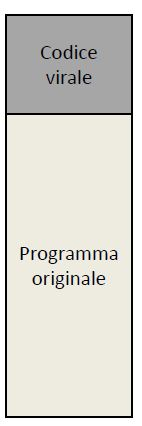
\includegraphics[height=5cm, width=8cm, keepaspectratio]{Immagini/Capitolo10/sicurezza_01.jpg}}
\subfigure[Circonda]
		{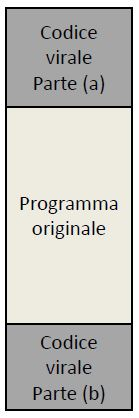
\includegraphics[height=5cm, width=8cm, keepaspectratio]{Immagini/Capitolo10/sicurezza_02.jpg}}
\subfigure[Integrato]
		{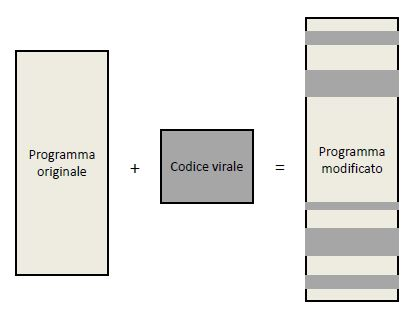
\includegraphics[height=5cm, width=8cm, keepaspectratio]{Immagini/Capitolo10/sicurezza_03.jpg}}
		\caption{Esempio grafico della posizione del codice malevolo \label{fig:virus_posizione_codice}}  
\end{figure}

\subsection{Firma del Virus}
Un virus non può essere completamente invisibile, il codice deve essere memorizzato da qualche parte e deve trovarsi in memoria per poter essere eseguito. Inoltre, il virus deve essere eseguito in modo particolare, con particolari metodi per la sua diffusione.
Ognuna di queste caratteristiche porta ad uno schema eloquente: \textbf{definizione} o \textbf{firma} del virus.
La definizione del virus viene utilizzata dagli analizzatori (antivirus) per rintracciarlo, può essere rilevato solo con la relativa definizione, ecco il perché dell'importanza dell'aggiornamento delle definizioni.
\newline
\subsubsection{Schemi di memorizzazione}
La maggior parte dei virus si associa a programmi archiviati su disco, il virus è invariabile perciò l'inizio del codice è una definizione rilevabile. Un altro parametro da rilevare può essere la dimensione del file a cui il virus si associa. Se il programma ospite  non viene modificato internamente, la sua dimensione complessiva aumenta.
Per non aumentare la dimensione è possibile  sostituire parti del programma, ma in questo caso l'ospite sarebbe modificato dal virus.
\newline
Anche in questo caso l'analizzatore di virus può sempre rilevare codice malevolo con un codice o un checksum per rilevare modifiche (può anche cercare degli schemi sospetti).
\subsubsection{Virus Polimorfico}
Per rendere difficoltosa la rilevazione del virus, il creatore può far si che lo schema di memorizzazione cambi. Si possono aggiungere delle operazioni, per rendere un virus polimorfico, come le seguenti:

\begin{itemize}

	\item Istruzioni che non fanno alcuna operazione (no-ops)
	\item Cambiare la posizione delle parti di codice rispetto a quelle di dati (se il programma malevolo è composto da 50 byte di codice e 100 di dati, si potrebbero inframezzare i byte di codice a quelli di dati in modo arbitrario)
	\item Crittografare parte del codice, sia le chiavi che le routine devono essere in chiaro per permettere la decrittazione. Non appena il virus viene eseguito, questi effettua la decifratura ottenendo la parte restante del suo codice eseguibile.
	
\end{itemize}

\section{Codice Malevolo Specializzato}
Finora abbiamo analizzato del codice anonimo, scritto per attaccare utenti e macchine in modo indiscriminato.
In questa sezione analizzeremo del codice malevolo scritto per un sistema in particolare, una applicazione specifica o per uno scopo ben determinato.
\subsection{Trapdoor}
Una trapdoor (botola) è un \textbf{punto di accesso non documentato} ad un modulo. Vengono utilizzate per lo sviluppo del codice, per provare il modulo, per lasciare agganci che permettono future modifiche e consentire l'accesso al modulo in caso di malfunzionamenti.
Oltre ciò, le trapdoor possono permettere l'accesso al programma una volta che questo viene messo in produzione.
\subsubsection{Stub e Codice Debug}
I sistemi informatici sono strutture complesse, per questa ragione i programmatori spesso sviluppano e provano i sistemi in modo metodico organizzato e modulare. I moduli vengono prima verificati singolarmente nella fase di \textbf{verifica dell'unità}. Successivamente vengono verificati nel funzionamento integrato, la \textbf{verifica di integrazione}.
Per la verifica dei singoli moduli e dei loro aggregati, potrebbero non essere disponibili i moduli che generano l'input o gestiscono l'output. Per questo motivo i programmatori realizzano delle routine aggiuntive che ricreano l'ambiente di esecuzione del modulo in esame. 
\newline
Gli stub verranno poi sostituiti, più avanti nella realizzazione, dai moduli di cui emulano le funzionalità.
Alle volte, quando l'origine di un problema in in un modulo non è evidente, il programmatore aggiunge codice di debug. Il codice serve per evidenziare cosa accade durante l'esecuzione, stampando valori di interesse o eseguendo speciali comandi.
\newline
Per controllare stub e codice di debug, il programmatore include sequenze di controllo speciali nella struttura del componente. L'inserimento dei comandi è una pratica di verifica riconosciuta, ma, se vengono lasciati in posizione dopo i test, i comandi aggiuntivi possono diventare un serio problema.
\subsubsection{Controllo degli Errori}
Un'altra fonte di trapdoor è uno scarso controllo degli errori; un buon sviluppatore progetta il sistema in modo che qualsiasi valore dei dati sia controllato prima del suo utilizzo. Il controllo comporta la verifica della correttezza del dato e della appartenenza all'intervallo previsto.
In sistemi progettati in modo scadente il controllo potrebbe non essere implementato e un dato fuori specifica potrebbe causare errori imprevisti.
\paragraph{Ad esempio} La falla di fingerd sfruttata dal worm Morris era di questo tipo. La routine di I/O di una libreria C non controlla se rimangono dati nel buffer di input prima di restituire il puntatore al carattere successivo.
\newline
Come i virus, le trapdoor non sono sempre cattive e possono rivelarsi utili anche per scoprire delle falle di sicurezza; perciò, affinché siano utili è indispensabile che:
\begin{itemize}
	\item siano documentate
	\item l'accesso sia strettamente controllato
	\item siano progettate ed utilizzate con la piena consapevolezza delle conseguenze
\end{itemize}

\subsubsection{Cause delle trapdoor}
Le trapdoor possono rimanere nei programmi di produzione perchè gli sviluppatori:
\begin{itemize}
	\item dimenticano di rimuoverle
	\item le lasciano intenzionalmente nel programma a scopo di test
	\item le lasciano intenzionalmente nel programma per la manutenzione
	\item le lasciano intenzionalmente nel programma per permettere accesso nascosto dopo che questo è diventato parte accettata di un sistema di produzione
\end{itemize}
In generale le trapdoor rappresentano una vulnerabilità quando espongono il sistema a modifiche durate l'esecuzione. Un sistema non è sicuro neanche quando qualcuno ritiene che nessun altro possa rilevare il varco!
\subsection{Salami Attack}
Deriva il suo nome dal modo in cui i pezzettini di carne e grasso vengono mischiati in una salsiccia o salame. Con la stessa tecnica un salami attack unisce bit di sequenze apparentemente non sequenziali per ottenere risultati significativi.
Il classico esempio di salami attack riguarda il calcolo di interessi bancari. Supposto che:
\begin{itemize}
	\item la banca paghi il 6.5\% di interesse annuo
	\item l'interesse viene calcolato su base mensile
	\item considerando un saldo di 100 \officialeuro, l'interesse mensile risulta di 0.5520 \officialeuro
	\item le banche effettuano i calcoli al centesimo di euro, cosa accade alle frazioni di centesimo?
\end{itemize}
Una popolare leggenda sulla sicurezza informatica narra di un programmatore che raccoglieva frazioni di centesimo e le accreditava sul suo conto.
In realtà, poiché alcuni arrotondamenti avvengono per difetto mentre altri per eccesso il saldo complessivo non dovrebbe scostarsi molto dallo zero.
\newline
Una situazione differente e molto redditizia, potrebbe essere ottenuta scalando qualche centesimo da ogni conto e transazione. Il correntista vedrebbe accreditarsi 0.53\officialeuro a posto di 0.55\officialeuro, probabilmente lo imputerebbe ad un proprio errore di calcolo, è comunque una questione di poco conto.
Oppure il programma potrebbe registrare un canone di 20\officialeuro mentre in realtà il costo è solo di 15\officialeuro, e accreditare la differenza su un conto speciale nascosto.
\subsubsection{Esistenza dei Salami Attack}
Perché i salami attack esistono ancora? I calcoli informatici sono notoriamente soggetti a piccoli errori relativi ad arrotondamento e troncamento. Anziché documentare esattamente i numerosi errori è più semplice accettare una piccola percentuale di errore come naturale ed inevitabile. 
Per far quadrare i conti, il programma include una correzione degli errori nei calcoli. Una \textbf{verifica inadeguata} di queste correzione è motivo per cui i salami attack ancora esistono e possono passare inosservati. 
Purtroppo il codice sorgente di un sistema è troppo grande o complesso per scovare attacchi di questo tipo, a meno che non vi sia un motivo per sospettarne la presenza. La dimensione ed il tempo sono punti a favore di chi programma codice malevolo!